\documentclass{beamer}
\usetheme{metropolis}
%\usepackage[backend=biber]{biblatex}
%\usepackage{booktabs} 
\usepackage{url}
\def\UrlBreaks{\do\/\do-}
\usepackage{amsfonts, amsmath, lmodern}
\usefonttheme{serif}
\usepackage{algorithm}
\usepackage{algorithmic}


%plots
\usepackage{tikz}
\usepackage{pgfplots}
\usepackage{pgfplotstable}
\pgfplotsset{compat=newest}
\usepackage{subcaption}
\usepackage{csvsimple}
%bibliography numbers
\setbeamertemplate{bibliography item}{\insertbiblabel}

\graphicspath{{./pictures}}
\setbeameroption{show notes} % comment out for the real presentation

\title{Fast Search of the Optimal Contraction Sequence in Tensor Networks}

\author{Max Koch, Christian Ortlepp}


\institute{Friedrich-Schiller-Universität Jena}

\date{20. Januar 2023}




\begin{document}

\begin{frame}
	\titlepage
\end{frame}

\begin{frame}{Gliederung}
	\tableofcontents
\end{frame}

\section{Einführung und Zielsetzung}
\begin{frame}{Einführung}
	TBD
\end{frame}

\section{Tensor-Kontraktionen}
\subsection{Allgemeines}

\begin{frame}{Begriffseinführungen}
	\begin{columns}
		\begin{column}{0.5\textwidth}
			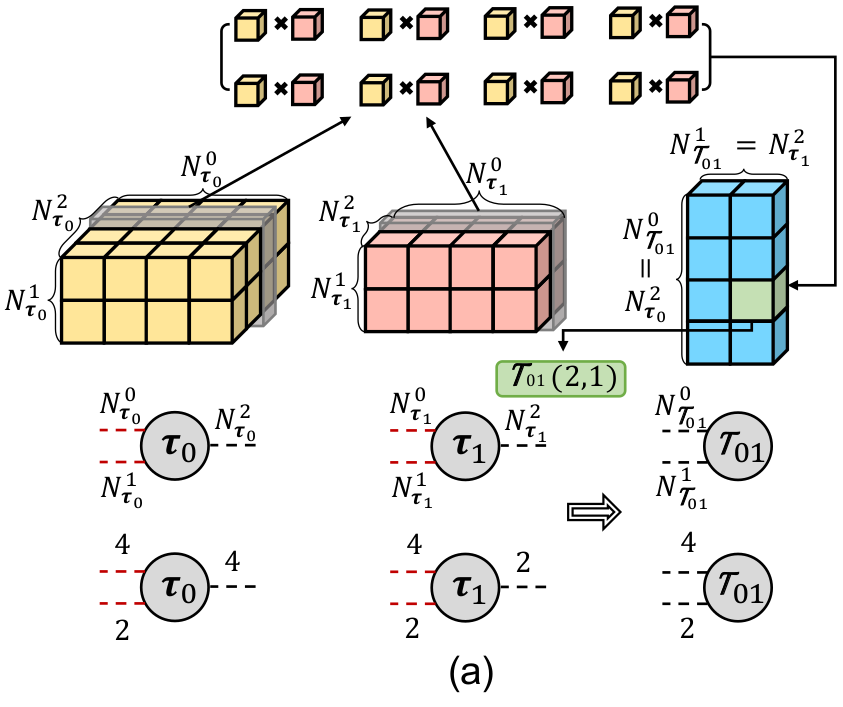
\includegraphics[scale=.2]{figure-2-a}
		\end{column}
		\begin{column}{0.5\textwidth}
			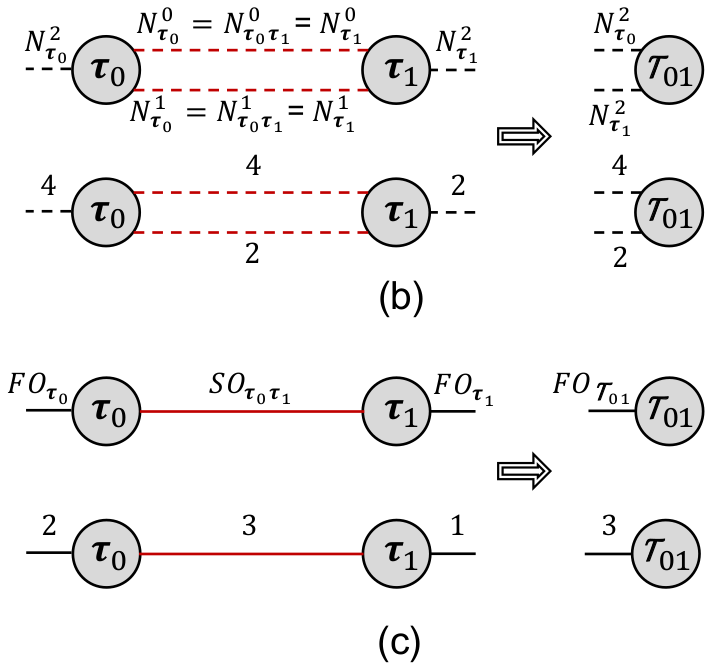
\includegraphics[scale=.2]{figure-2-b}
		\end{column}
	\end{columns}
\end{frame}
\note[itemize]{
	\item Graph-Notation: Kanten=Dimensionen (Order), Knoten=Tensoren
	\item Kanten zwischen Knoten "Sharing Orders", sonst "Free Orders"
	\item Kantengewicht: $\log_2$ der Order
	\item bei $V$ Tensoren werden $V-1$ Schritte benötigt
}

\begin{frame}{Kontraktion}
	\begin{columns}
		\begin{column}{0.5\textwidth}
			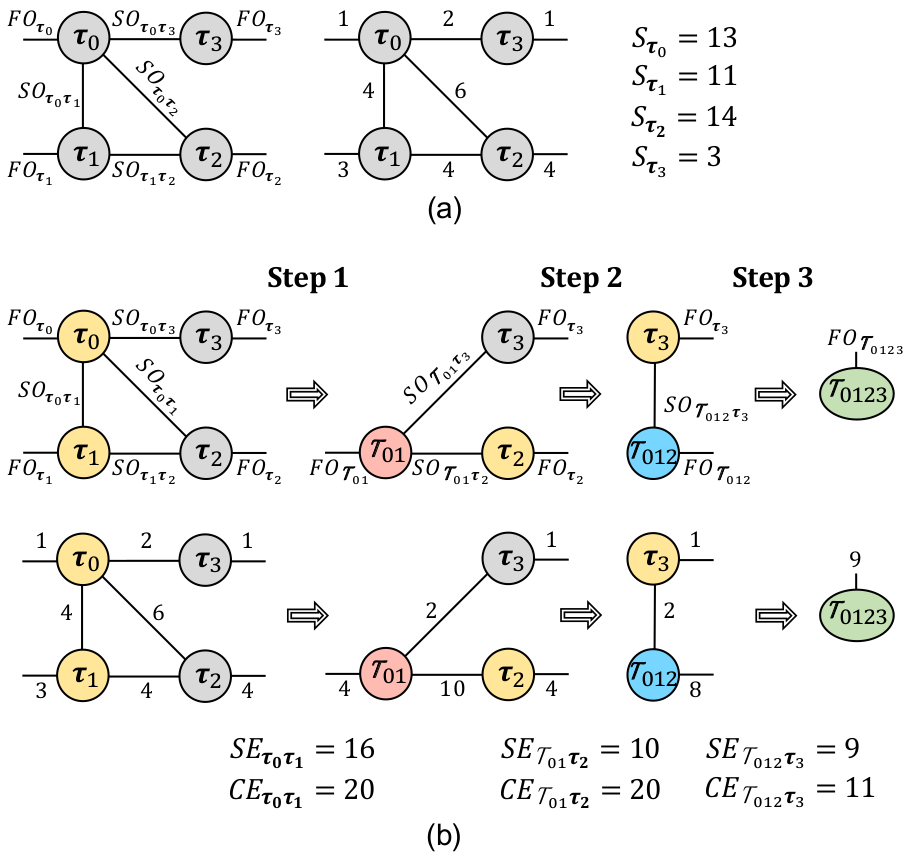
\includegraphics[scale=.17]{figure-3-a}
		\end{column}
		\begin{column}{0.5\textwidth}
			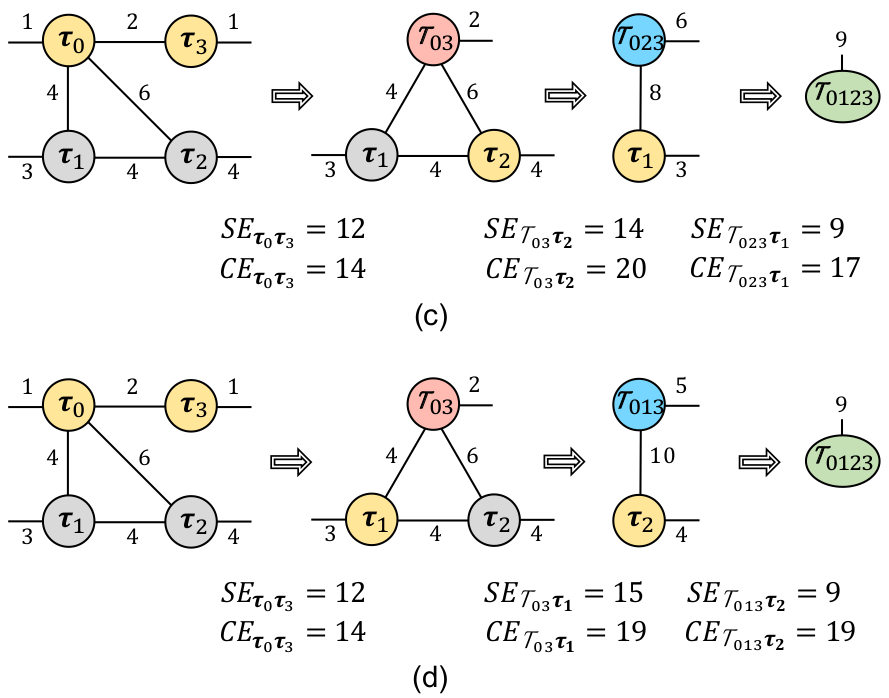
\includegraphics[scale=.17]{figure-3-b}
		\end{column}
	\end{columns}
\end{frame}
\note[itemize]{
	\item verschiedene Kontraktionsreihenfolgen
	\item bei jedem Schritt wird eine sharing order eliminiert
}

\subsection{BFS-Algorithmus}
\begin{frame}{BFS - Einführung}
	\begin{itemize}
		\item BFS = Breadth First Search
	\end{itemize}
\end{frame}
\note[itemize]{
	\item man fängt mit 2er kombinationen der Tensoren an, berechnet jeweils MS und MC
	\item dann geht man zur nächst größeren Menge (3er, 4er, 5er ... Kombinationen) und macht dasselbe, dabei verwendet man die bereits berechneten Ergebnisse wieder
	\item wenn man alle durch is sucht man das Minimum der in der letzen Iteration berechneten Werte
	\item MS und MC berechenen mit Formel aus vorherigem Kapitel
	\item Suchraum: $O(2^v)$
}


\section{Adjazenzmatrix-basierte Kontraktionssuche}

\subsection{Vanilla - Suche}
\begin{frame}{Sharing Order Calculation}
	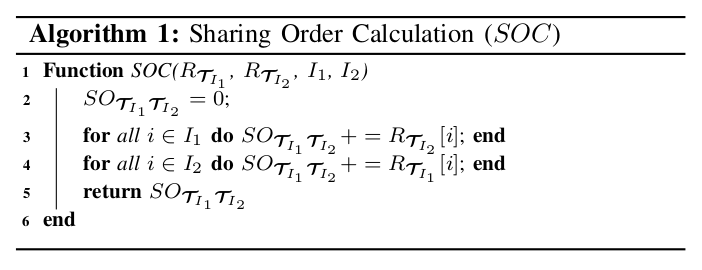
\includegraphics[scale=0.4]{algorithm-1}
\end{frame}
\note[itemize]{
	\item WICHTIG: ab jetzt arbeiten wir auf den Adjazenzmatrizen und nicht auf den tensoren selbst
	\item input:
	\item zwei zeilen-vektoren  der  Matrizen zu kontrahierenden Tensoren
	\item die Menge der Tensoren, aus welchen die inputs (durch vorherige Kontraktionen) entstanden sind
}
\begin{frame}{Vanilla Suche - Teil 1}
	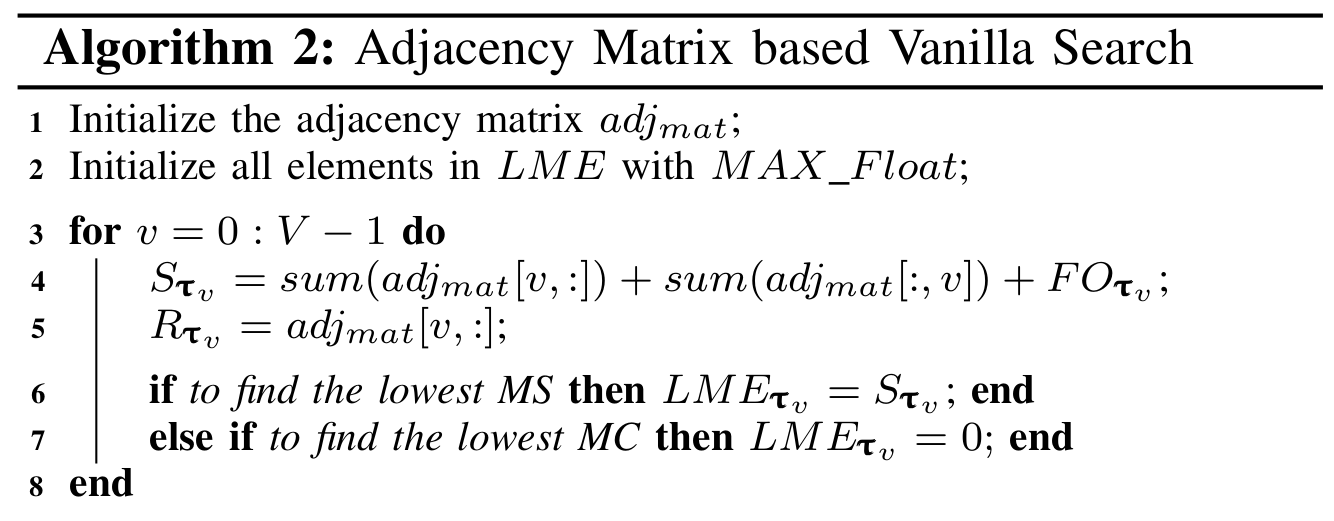
\includegraphics[scale=0.2]{algorithm-2-a}
\end{frame}
\note[itemize]{
	\item 1-2: initialisiere Adjazenzmatrix und Lowest Maximum Expense für alle tensoren
	\item 3: iteriere über alle Tensoren im Netzwerk
	\item 4: speichere die Größe des Tensors (Data Size)
	\item 5: speichere Zeilenvektor aus Adjazenzmatrix
	\item 6-7: Je nach modus (compute/storage) wird LME unterschiedlich initialisiert
}
\begin{frame}{Vanilla Suche - Teil 2}
	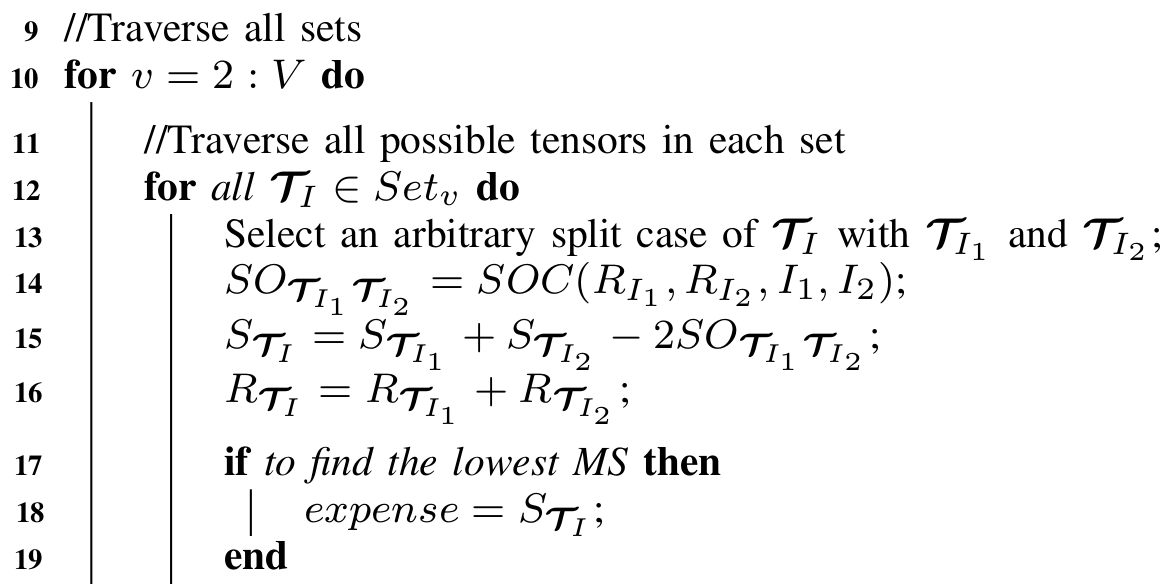
\includegraphics[scale=0.25]{algorithm-2-b}
\end{frame}
\note[itemize]{
	\item 10: iteriere über möglichen Kontraktions-Größen
	\item 12: iteriere über alle Tensoren im Set. Größe des aktuellen Tensor: $S_{T_I}$, Repräsentation dieses Tensors als Zeilenvektor: $R_{T_I}$
	\item 13: wähle beliebig einen split-case des aktuellen Tensors $T_I$
	\item 15-16: berechne den Zeilenvektor und Data Size von $T_I$
	\item 17: Falls neues MS gefunden wurde wird dies gespeichert
	\item Generell: initialisiert nur variablen, die tatsächliche Berechnung geschieht in Teil 3
}
\begin{frame}{Vanilla Suche - Teil 3}
	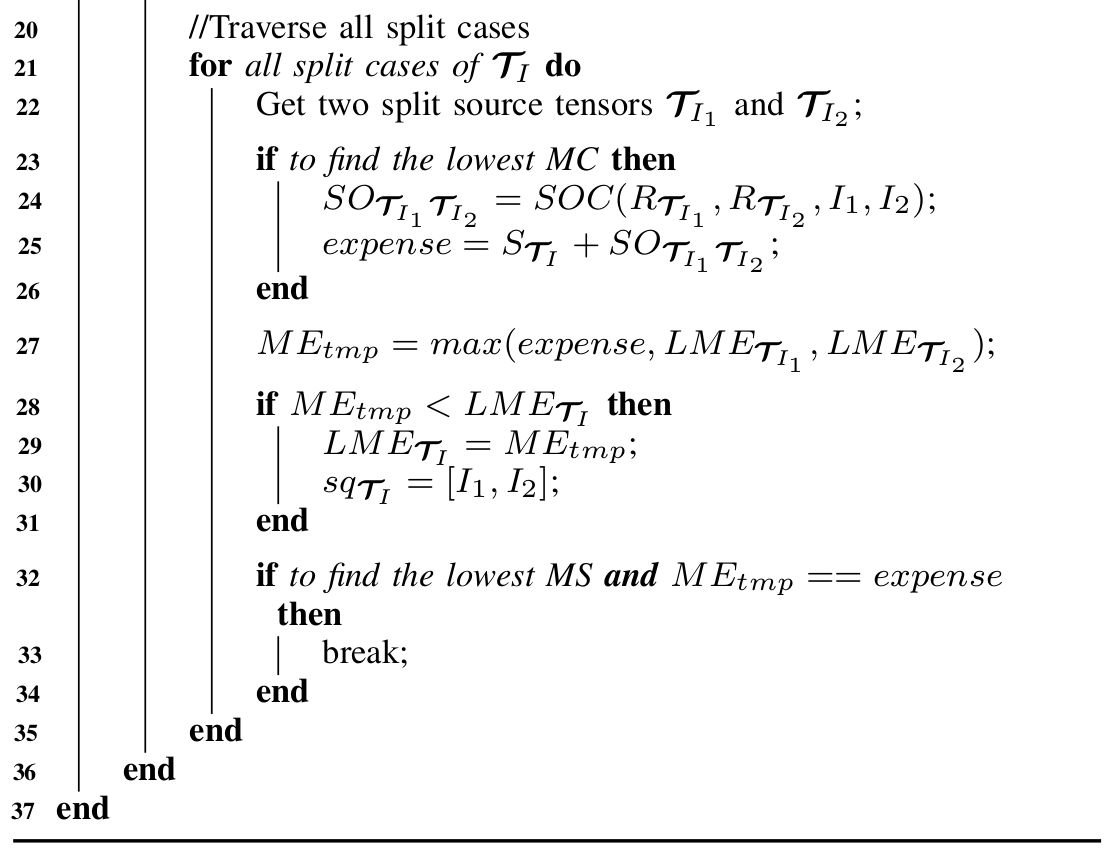
\includegraphics[scale=0.25]{algorithm-2-c}
\end{frame}
\note[itemize]{
	\item WICHTIG: immernoch innerhalb der vorherigen beiden Schleifen
	\item 21: Iteriere über jeden split case von $T_I$
}


\subsection{Outer Product Pruning}
\begin{frame}{Pruning - Einührung}
	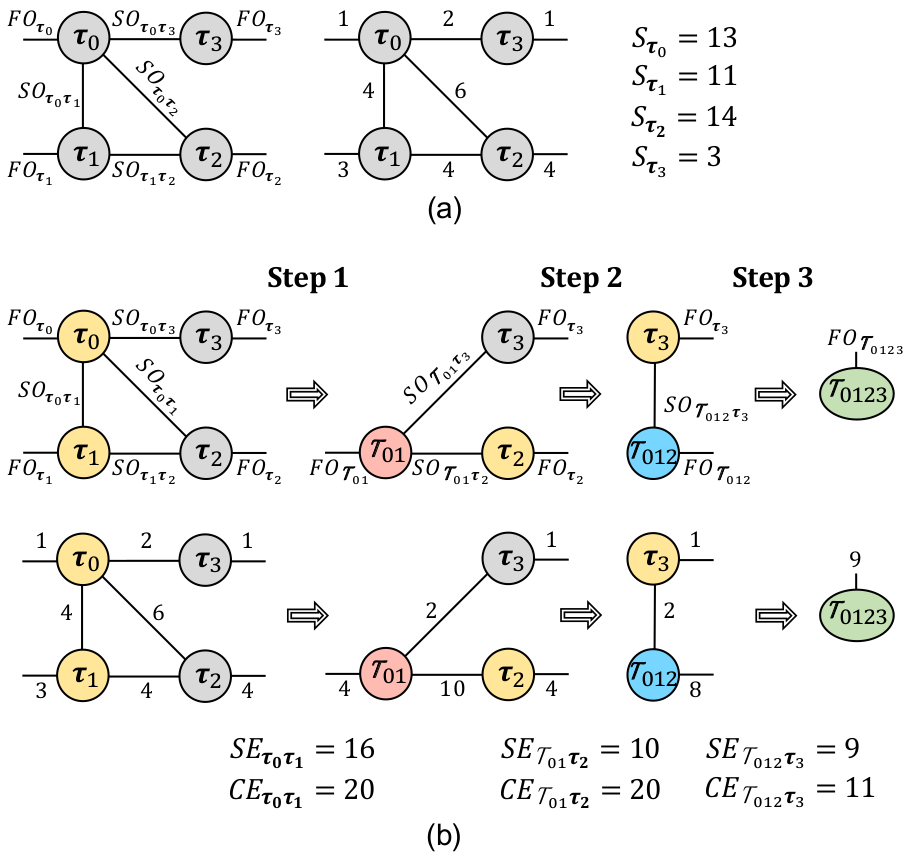
\includegraphics[scale=0.2]{figure-3-a}
\end{frame}
\note[itemize]{
	\item outer product: multiplikation von Tensoren ohne sharing Orders (siehe $\tau_2, \tau_3$)
	\item es ist bewiesen dass die beste Kontraktion (kleinste MS / MC) immer ohne outer - products auskommt
	\item[$\Rightarrow$] Outer products können bei Kontraktionen ausgeschlossen werden
	\item Wenn es im Netzwerk "Subnetzwerke" gibt, welche untereinander keine sharing orders teilen, kann in den subnetzwerken unabhängig voneinander nach der optimalen sequenz gesucht werden
}
\begin{frame}{Pruning - Einführung}
	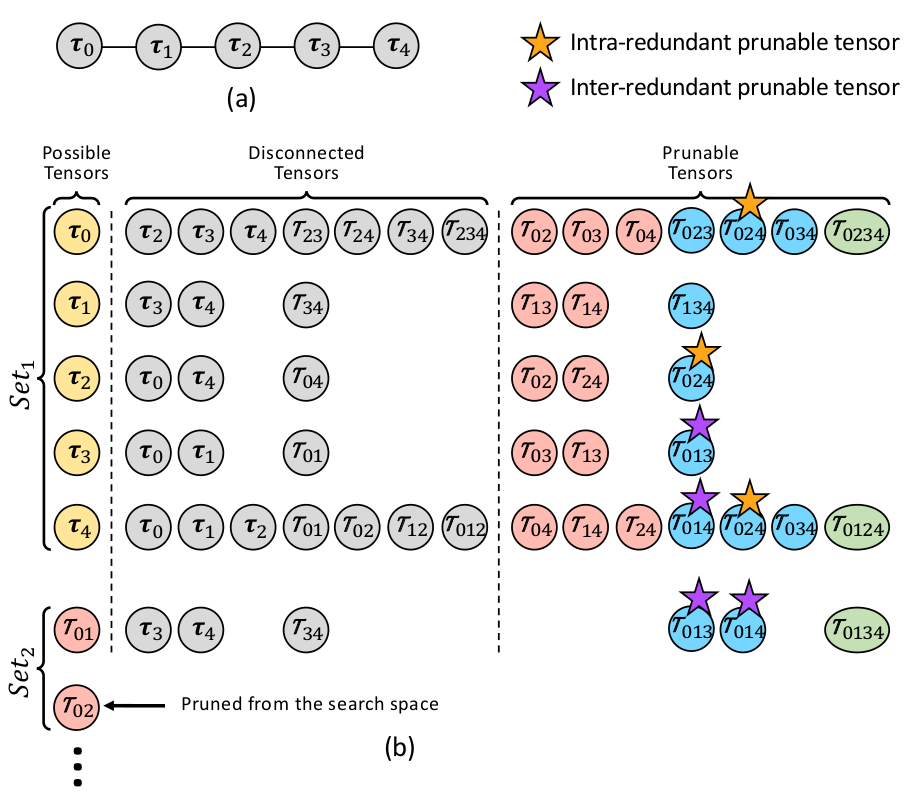
\includegraphics[scale=0.25]{figure-6}
\end{frame}
\note[itemize]{
	\item TODO Figure 5 Adjazenzmatrix Struktur
}
\begin{frame}{Pruning - Algorithmus}
	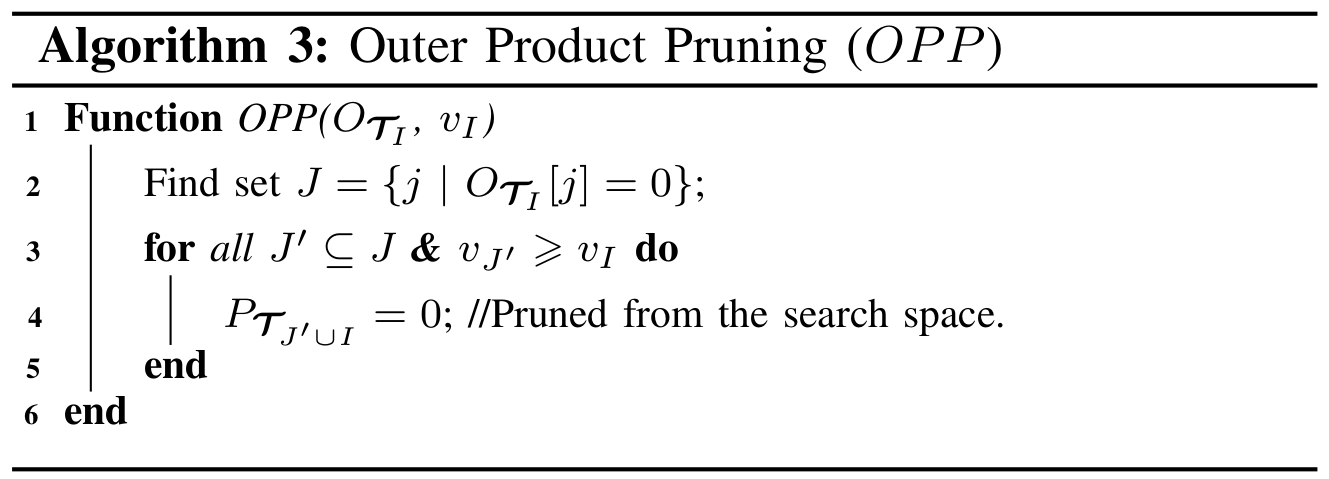
\includegraphics[scale=0.25]{algorithm-3}
\end{frame}
\note[itemize]{
	\item someNote
}
\section{Ergebnisse}

\begin{frame}{Suche mit Pruning}
	\begin{itemize}
		\item getestet auf verschiedenen Topologien (Kette, Baum, Radial und Gitter)
		\item Anzahl zusätzlicher Kanten variabel
	\end{itemize}
\end{frame}
\note[itemize]{
	\item someNote
}
\begin{frame}{Suche mit Pruning - Baseline}
	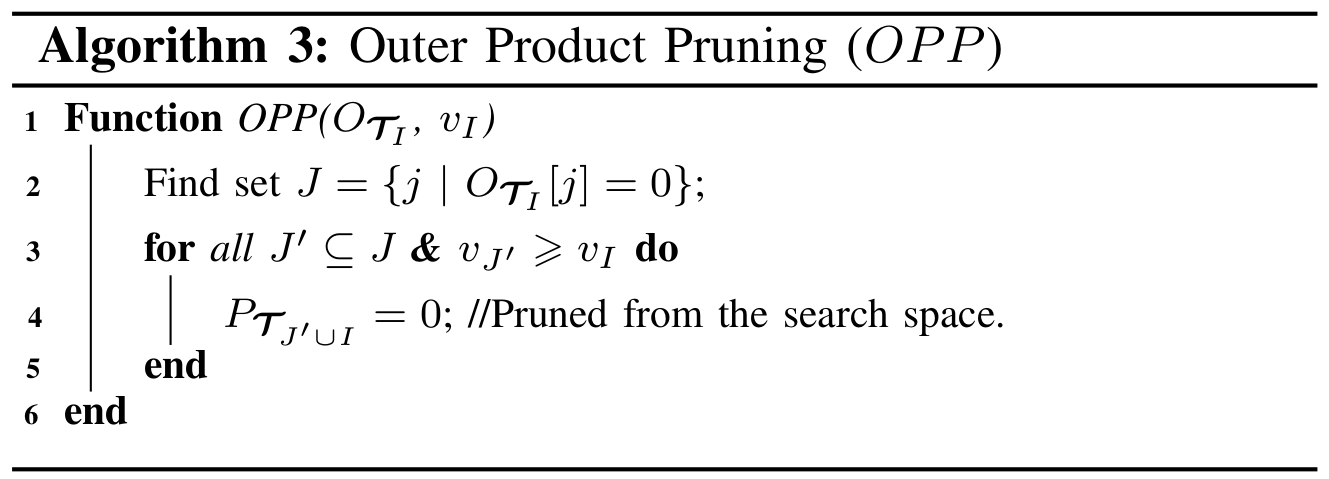
\includegraphics[scale=0.25]{table-3}
\end{frame}
\note[itemize]{
	\item 19 Tensoren, keine zusätzlichen Kanten
	\item pruning verbessert Suchzeiten, bei MC effektiver als bei MS
	\item Kette ist besser als Baum ist besser als Radial
}
\begin{frame}{Suche mit Pruning - Vergleich}
	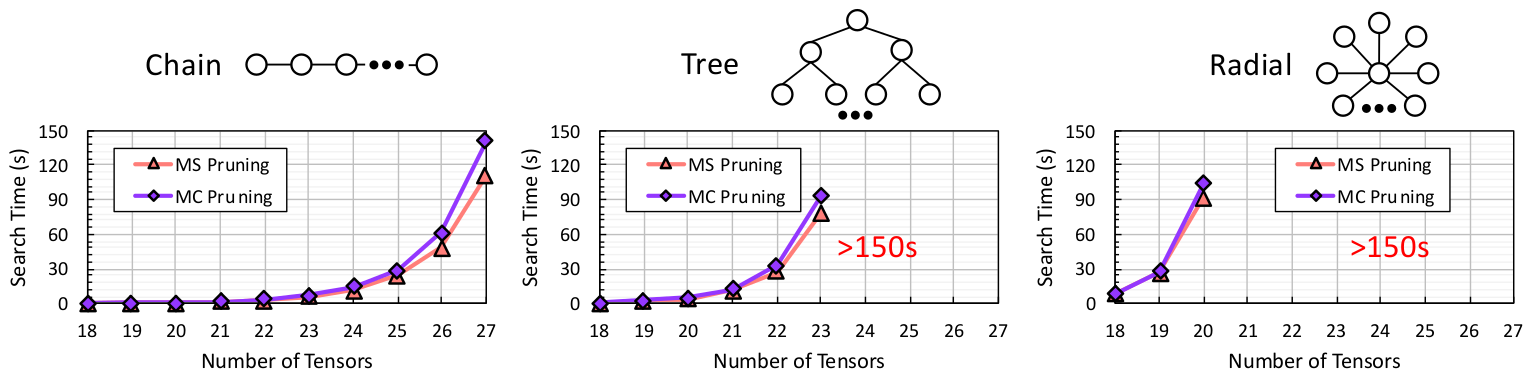
\includegraphics[scale=0.2]{figure-9}
	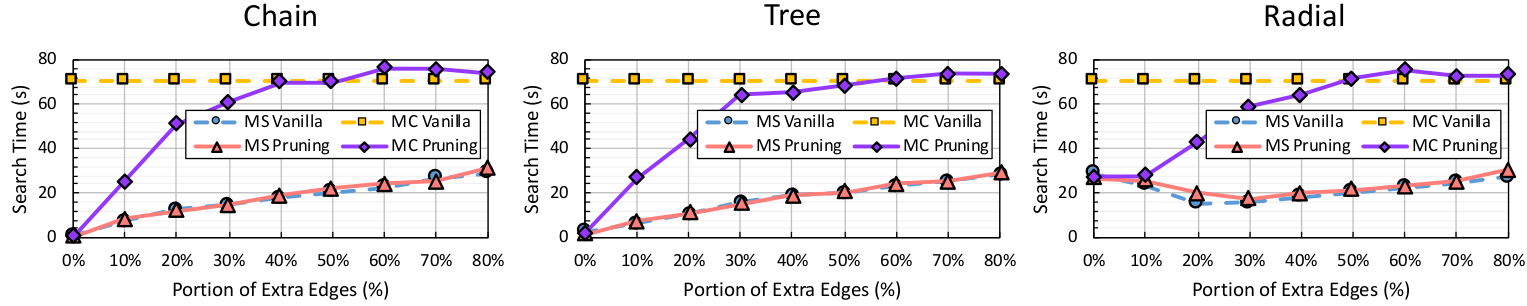
\includegraphics[scale=0.2]{figure-10}
\end{frame}
\note[itemize]{
	\item fig 9: Vergleich MS vs MC auf verschiedenen Topologien
	\item bei Baum und Radial abgheschnitten da zu lange suchzeiten (> 150s)
	\item Kette: hat die meisten prunable tensors, deswegen ist es dort am effektivsten
	\item 
}


\begin{frame}[allowframebreaks]{Bibliography}
	\bibliography{../bibliography/bibliography.bib}
	\bibliographystyle{splncs04}
	\nocite{*}
\end{frame}

\end{document}
